\documentclass[12pt, openany]{report}
\usepackage[utf8]{inputenc}
\usepackage[T1]{fontenc}
\usepackage{amsmath,amsfonts,amssymb}
\usepackage{amssymb}
\usepackage{multicol}
\usepackage[a4paper,left=2.5cm,right=2.5cm,top=2.5cm,bottom=2.5cm]{geometry}
\usepackage[english]{babel}
\usepackage{libertine}
\usepackage{graphicx}
\usepackage{wrapfig}
\usepackage{algorithm}
\usepackage{algpseudocode}
\usepackage{float}
\usepackage{enumitem}
\usepackage{pythonhighlight}
\usepackage[]{titletoc}
\usepackage{empheq}
\usepackage{titlesec}
\usepackage{qtree}
\usepackage{mathpazo}
\usepackage{xfrac}
\usepackage{textcomp}
\usepackage{mathtools}
\usepackage{tikz}
\usetikzlibrary{arrows.meta, positioning}
\usepackage{caption}
\usepackage{tabularray}
\usepackage{subcaption}
\usepackage[bottom]{footmisc}
\usepackage{pdfpages}
\usepackage{tabularx}
\usepackage{amsthm}
\usepackage[skins]{tcolorbox}
\titleformat{\chapter}[display]
  {\normalfont\bfseries}{}{0pt}{\Huge}
\usepackage{hyperref}
\newcommand{\hsp}{\hspace{20pt}}
\newcommand{\HRule}{\rule{\linewidth}{0.5mm}}
\newcommand{\R}{\mathbb{R}}
\newcommand{\N}{\mathbb{N}}
\newcommand{\C}{\mathbb{C}}
\newcommand{\E}{\mathbb{E}}
\theoremstyle{definition}
\newtheorem{thm}{Theorem}[chapter]
\newtheorem{definition}[thm]{Definition}
\newtheorem{lem}[thm]{Lemma}

\hbadness=100000
\begin{document}
\begin{titlepage}
    \begin{sffamily}
    \begin{center}
        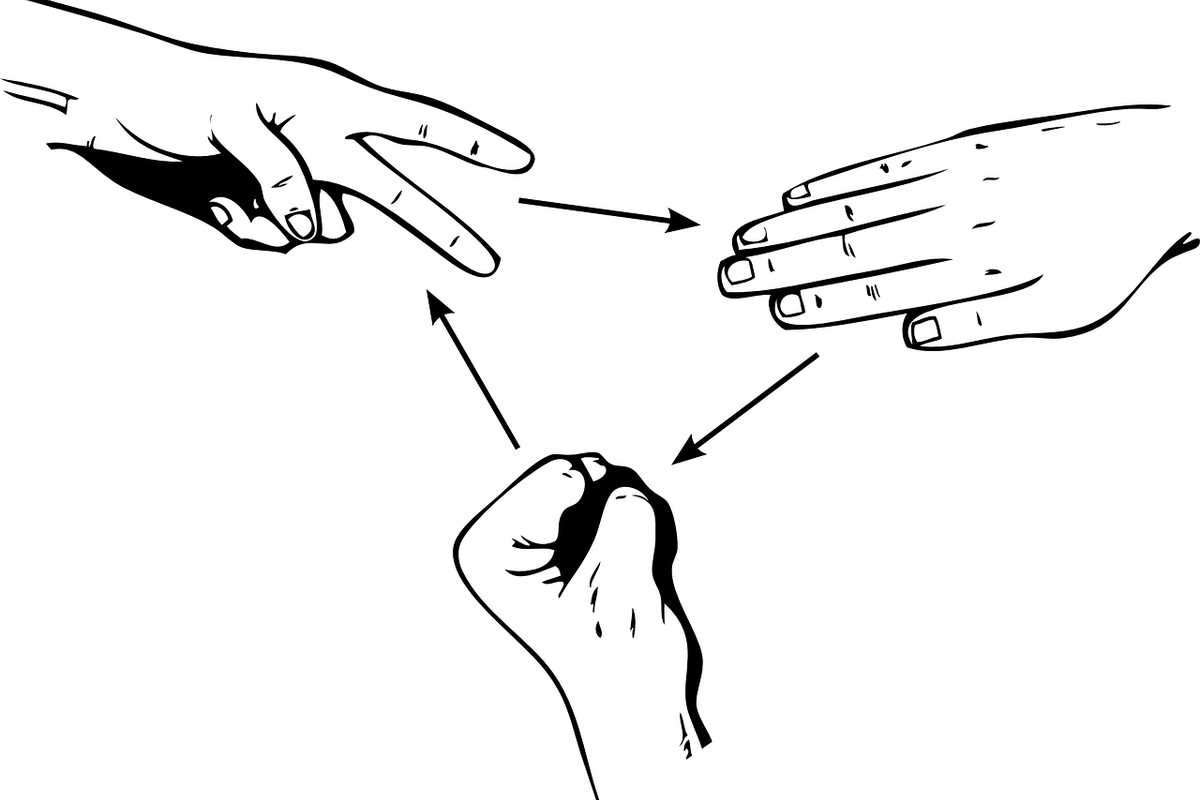
\includegraphics[scale=0.25]{img/page_de_garde.png} \\[1cm]
        \HRule \\[0.4cm]
        { \huge \bfseries LINMA2111 - Discrete mathematics II \\[0.4cm] }
    
        \HRule \\[1.5cm]
        \textsc{\LARGE Simon Desmidt\\ Issambre L'Hermite Dumont}\\[1cm]
        \vfill
        \vspace{2cm}
        {\large Academic year 2025-2026 - Q1}
        \vspace{0.4cm}
         
        
\includegraphics[width=0.15\textwidth]{img/epl.png}
        
        UCLouvain\\
    
    \end{center}
    \end{sffamily}
\end{titlepage}

\setcounter{tocdepth}{1}
\tableofcontents
\chapter{Introduction}
\section{Sorting problems}
\subsection{Introduction}
A sorting problem is a problem that consists of taking a sequence of $n$ objects and putting them in order. This kind of problem is made of three main elements:
\begin{itemize}
  \item Context: set $S$ with a partial order $<$;
  \item Input: $n$ elements of $S$;
  \item Output: permutation of the input elements respecting the order.
\end{itemize}
To prove the correctness of an algorithm, we generally use the Hoare triple, i.e. a tuple for any input array $x_0$:
\begin{equation}
  \begin{aligned}
	&\{\text{Algorithm to be used};\ \text{Precondition}; \ \text{Postcondition}\}\\
	&\left\{IS;\ x=x_0;\ x\text{ is sorted and is a permutation of }x_0\right\}
\end{aligned}
\end{equation}
where IS is the insertion sort algorithm, and $x$ is the sorted array. From now on, we will call "sorting" a sorted permutation. \\
In practice, to prove the correctness of an algorithm, we define the invariant and the base case, and do an induction step show that the invariant is preserved.\\
\subsection{Definition of complexity}
For some functions $f,g:\mathbb{N} \to \R^+$, 
\begin{equation}
  	\begin{aligned}
		&f\in \mathcal{O}(g) \Longleftrightarrow \exists c>0, \exists n_0, \forall n>n_0,\ f(n)\le cg(n)\\
		&f\in \Omega(g)\Longleftrightarrow g\in \mathcal{O}(f)\\
		& f\in \Theta(g)\Longleftrightarrow f\in \mathcal{O}(g)\text{ and } f\in \Theta(g)\\
		&f\in o(g) \Longleftrightarrow \exists c>0, \exists n_0, \forall n>n_0,\ f(n)< cg(n)\\
		&f\in \omega(g)\Longleftrightarrow g\in o(f)\\
  	\end{aligned}
\end{equation}
\begin{itemize}
	\item The time complexity is the number of operations as a function of the input size;
	\item The space complexity is the amount of memory used (in addition to the input) as a function of the input size. 
\end{itemize}
We define the average case complexity as an expectation of the time taken by the algorithm on each input possible, with a dependence in the size of the input.
\begin{equation}
	t = \mathbb{E}_{x\sim D}[T(x)]
\end{equation}
where $D$ is the distribution of the input.\\
\subsection{Divide and conquer}
The divide and conquer method consists in three steps:
\begin{enumerate}
	\item Divide: create smaller subproblems;
	\item Recurse: solve them;
	\item Combine: merge the solutions.
\end{enumerate}
In sorting problems, a divide-and-conquer algorithm is the merge sort algorithm. It consists in dividing the array in two, sorting each half recursively, and merging the two sorted halves. The merge operation is done in linear time.\\
\section{Complexity of sorting algorithms}
No sorting algorithm can be faster than $\Omega(n \log(n))$. This can be proven through the complexity of comparison-based algorithms. 
\chapter{Divide-and-conquer algorithms}
\section{Complexity of a multiplication}
Given two $n$-digit numbers, we want to compute their product:
\begin{equation}
  	\begin{cases}
		a = a_{n-1}a_{n-2}...a_1a_0\\
		b = b_{n-1}b_{n-2}...b_1b_0\\
  	\end{cases}
	\Longrightarrow c=a\cdot b = c_{2n-1}...c_0
\end{equation}
Let us define $B$ as the basis (e.g. 10) and decompose $a$ and $b$ in two parts:
\begin{equation}
	\begin{cases}
		a = \alpha_0+B\alpha_1\\
		b = \beta_0+B\beta_1
	\end{cases} \Longrightarrow a\cdot b = \alpha_0\beta_0 + B(\alpha_1\beta_0 + \alpha_0\beta_1)+B^2 \alpha_1\beta_1
\end{equation}
In that case, we find a recurrence relation for the computation time:
\begin{equation}
	T(n) = 4T(n/2) + \Theta(n)
\end{equation}
We introduce the Master theorem to solve this equation, see section below. It gives a complexity of $T(n) = \Theta(n^{\log_2(4)}) = \Theta(n^2)$.\\
To reduce the complexity, we can change the value of the parameter $a$ from 4 to 3 by calculating only 3 products:
\begin{equation}
	\begin{cases}
		\gamma_0 = \alpha_0\beta_0\\
		\gamma_2 = \alpha_1\beta_1\\
		\gamma_1 = (\alpha_0+\alpha_1)(\beta_0+\beta_1)-\gamma_0-\gamma_2\\
	\end{cases}
\end{equation}
This reduces the complexity to $\Theta(n^{1.58})$. \\
Following a similar reasoning, we can instead divide $a$ and $b$ into 3 sums instead of 2, and get 5 multiplications. This gives a complexity of $\Theta(n^{\log_3(5)}) = \Theta(n^{1.46})$. Dividing in 4, 5, etc, we converge to a complexity of $\Theta(n)$ and this is the optimal complexity for the multiplication of two numbers of $n$ digits. The problem is that the constant in front of the $n$ starts to grow as we divide into more and more limbs, and so a bigger exponent can be enough for most arrays\footnote{We call galactical algorithm an algorithm that is asymptotically good but the constant grows so large that it is only useful for huge arrays (e.g. $\sim10^{80}$).}.
\section{Master Theorem} 
Let $a\ge 1$ and $b>1$ be constants and $f(n)$ a positive function, and let $T(n)$ be defined by $T(0)>0$ and $T(n) = aT(\lfloor n/b\rfloor)+f(n)$. Then,
\begin{itemize}
	\item If $f(n) = \mathcal{O}(n^{\log_b (a)-\epsilon})$ for some $\epsilon>0$, then $T(n) = \Theta(n^{\log_b(a)})$;
	\item If $f(n) = \Theta(n^{\log_b(a)})$, then, $T(n) = \Theta(b^{\log_b(a)}\log(n))$;
	\item If $f(n) = \Omega(n^{\log_b(a)+\epsilon})$ for some $\epsilon>0$ and if, for some $c>1$ and $n_0$ such that $af(\lfloor n/b\rfloor)\le cf(n)$ for all $n\ge n_0$, then $T(n)=\Theta(f(n))$;
\end{itemize}
\subsection{Proof}
\Tree [.{$n=b^k$} 
        [.{$\phantom{X}$} 
            [.{$\vdots$} {$\phantom{X}$} {$\phantom{X}$} ]
            [.{$\vdots$} {$\phantom{X}$} {$\phantom{X}$} ]
        ]
        [.{$\phantom{X}$} 
            [.{$\vdots$} {$\phantom{X}$} {$\phantom{X}$} ]
            [.{$\vdots$} {$\phantom{X}$} {$b^0$} ]
        ]
    ]

In that tree, for a level $i$, the size of the problem is $b^i$ and the number of subproblems is $a^{k-i}$. By summing up, 
\begin{equation}
	T(b^k) = \sum_{i=0}^k a^{k-i}f(b^i)
\end{equation}
For a function $f(n)=n^\alpha$, 
\begin{equation}
	T(n) = a^k \sum_{i=0}^k \left(\frac{b^\alpha}{a}\right)^i = a^k \frac{1-(\frac{b^\alpha}{a})^{k+1}}{1-b^\alpha/a}
\end{equation}
Under the assumption that $\alpha \neq \log_b(a)$. As $k=\log_b(n)$, we can replace above and simplify using the formula $a^{\log_b(n)} = n^{\log_b(a)}$. In the case where $a=b^\alpha$, then 
\begin{equation}
	T(n) = a^k (k+1) = a^{\log_b(n)} (\log_b(n)+1) = \Theta(n^{\log_b(a)}\log(n))
\end{equation}
\section{Multiplying polynomials}
Consider $a(x) = a_0+a_1x+a_2 x^2 + \dots + a_{n-1}x^{n-1}$. It can either be represented by its coefficients, or some values $(a(x_0),\dots, a(x_{n-1}))$ for $n$ distinct values. To compute those values, we can use a matrix-vector product:
\begin{equation}
	\begin{bmatrix}
		1 & x_0 & \dots & x_0^{n-1}\\
		\vdots & \vdots & \ddots & \vdots \\
		1 & x_{n-1} & \dots & x_{n-1}^{n-1}\\
	\end{bmatrix}\begin{bmatrix}
		a_0 \\ \vdots \\ a_{n-1}
	\end{bmatrix} = Va
\end{equation}
where the matrix $V$ is called the Vandermonde matrix. 
\subsection{Convolution theorem}
\begin{center}
	\begin{tikzpicture}[node distance=4cm, auto, font=\small]
		
		% Nodes
		\node[draw, red, thick, rectangle, inner sep=8pt] (A) {\textcolor{black}{
			$\begin{aligned}
				a(x) &= \sum_i a_i x^i \\ 
				b(x) &= \sum_i b_i x^i
			\end{aligned}$}
			};
			
			\node[draw, red, thick, rectangle, inner sep=8pt, right=of A] (B) {
				\textcolor{black}{$c(x) = \sum_i c_i x^i$}
				};
				
				\node[draw, red, thick, rectangle, inner sep=8pt, below=of A] (C) {
					\textcolor{black}{$\begin{matrix}
						a(x_0) & \dots & a(x_{2n-1}) \\
						b(x_0) & \dots & b(x_{2n-1})
					\end{matrix}$}
					};
					
					\node[draw, red, thick, rectangle, inner sep=8pt, right=of C] (D) {
						\textcolor{black}{$c(x_0) \dots c(x_{2m-1})$}
						};
						
				% Arrows
				\draw[->, red, thick] (D) -- (B) node[midway, above] {\small \textcolor{black}{Interpolate $V^{-1}$}};
				\draw[->, red, thick] (A) -- (C) node[midway, left] {\small \textcolor{black}{Evaluate $V$}};
				\draw[->, red, thick] (C) -- (D) node[midway, below] {\small \textcolor{black}{pointwise mult}};
						
	\end{tikzpicture}
\end{center}
This method gives bad conditioning, but this is not a problem here as we consider integer matrices. 
\subsection{Discrete Fourier Transform}
If we take the points as the $n$ complex roots of 1, i.e. $x_0 = e^{2\pi i/n}$ and $x_j = e^{2\pi ij/n}$, then we get a Discrete Fourier Transform matrix. Defining $\omega_n = x_0$,
\begin{equation}
	V = \begin{bmatrix}
			1 & 1 & 1 & 1 \\
			\vdots & \omega_n & \dots & \omega_n^{n-1}\\
			\vdots & \ddots & \omega_n^{(i-1)(j-1)} & \vdots \\
			1 & \omega_n ^{n-1} & \dots & \omega_n^{(n-1)^2}
		\end{bmatrix}
\end{equation}
This gives us 
\begin{equation}
	V^{-1} = \frac{1}{n} \begin{bmatrix}
		\omega_n^{-(i-1)(j-1)}
	\end{bmatrix}
\end{equation}
and so $V = \frac{1}{n}V^*$.
\end{document}